\section{Описание алгоритмов сортировок}

\subsection{Чётно-нечётная сортировка}
Алгоритм сортировки построен на другой сортировке - пузырьковой. В отличие от него независимо
сравниваются элементы под чётными и нечётными индексами с последующими элементами независимо.
В начале итерации флаг, определяющий отсортирован ли массив, ставится как истинна, а далее каждый
нечётный сравнивается с последующими, и если необходимо поменять местами, то в флаг устанавливается
ложь. Аналогично для чётных. Алгоритм прекращается, когда флаг остаётся истинным. Сложность сортировки:
\begin{itemize}
  \item худшая - $O(n^2)$.
  \item средняя - $O(n^2)$.
  \item лучшая - $O(n)$.
\end{itemize}

\begin{figure}[H]
  \centering
  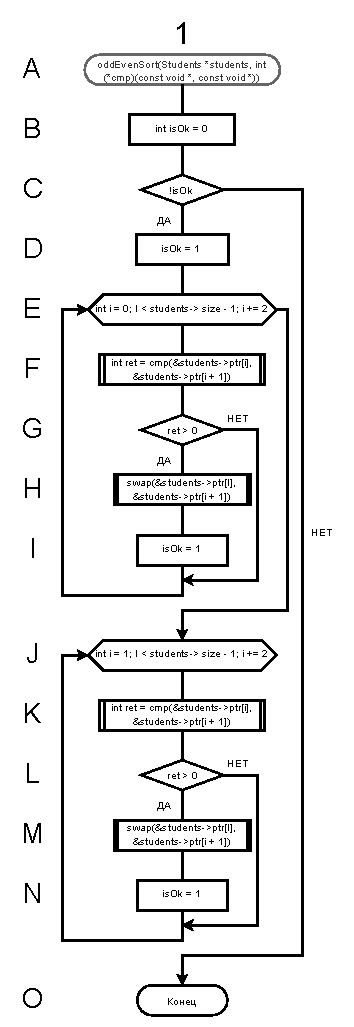
\includegraphics[width=0.475\textwidth]{fun_oddEvenSort}
  \caption{Блок-схема алгоритма работы функции \texttt{oddEvenSort()}}
\end{figure}

\subsection{Двухсторонняя сортировка выбором}

Алгоритм сортировки построен на другой сортировке - сортировкой выбором. Помимо максимального
элемента массива будет находиться и минимальный. Максимум будет перемещаться в конец подмассива,
а минимум соотвественно в начало. Сложность сортировки:

\begin{itemize}
  \item худшая - $O(n^2 / 2)$.
  \item средняя - $O(n^2 / 2)$.
  \item лучшая - $O(n^2 / 2)$.
\end{itemize}

\begin{figure}[H]
  \centering
  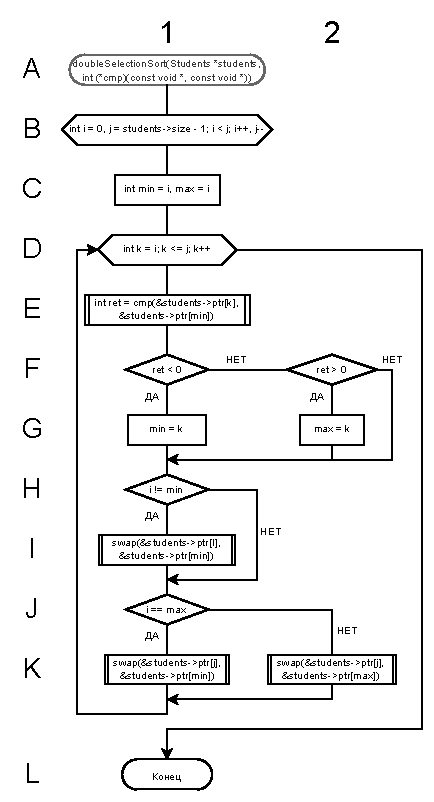
\includegraphics[width=0.55\textwidth]{fun_doubleSelectionSort}
  \caption{Блок-схема алгоритма работы функции \texttt{doubleSelectionSort()}}
\end{figure}
